\chapter{istar::USR: ultrafast shape recognition}

\section{Abstract}

Finding structurally similar compounds to a query ligand has been an important but daunting problem for a long time.

This is an ongoing collaborative project with Pedro J. Ballester from European Bioinformatics Institute, Cambridge, United Kingdom.

\section{Introduction}

Molecular shape has been widely acknowledged as a key factor for biological activity and thus is regarded as a very important pattern for which to search. Searching the molecular database for compounds that most closely resemble the shape of a given query molecule, be it a known inhibitor of a target protein, a natural product, or even a patented compound, finds pragmatic applications in ligand-based virtual screening \citep{1332,1380} and target fishing \citep{1408,1402}. Therefore molecular similarity search assists in discovering structurally novel active compounds, or in identifying potential interacting target of bioactive ligands, which is useful for understanding the polypharmacology and safety profile of existing drugs. Furthermore, this approach can be extended to other scientific disciplines such as designing content-based Internet search engines for 3D geometrical objects or performing similarity comparisons between proteins \citep{1280}.

The molecular shape similarity can be quantified by methods based on structural alignment \citep{1440,887,1439} or shape recognition \citep{1379,1338,1331}. Structural alignment is also known as molecular superposition and requires precise geometric comparison which is often computationally intensive. Shape recognition, on the other hand, encodes shape information into a numerical feature vector, which can be subsequently used to compute a similarity score between two molecules very efficiently.% \citep{} Bioactive molecules: perfectly shaped for their target

USR (Ultrafast Shape Recognition) \citep{1379} was the very first non-superposition method for molecular shape comparison, and demonstrated superior computational performance at least three orders of magnitude faster than previously existing alignment-based methods. USR has another major advantage of being invariant to spatial orientation and translation, and hence circumvents the problematic requirement of aligning molecules. USR defines the shape of a molecule independently and for every molecule uses a fixed set of 12 descriptors derived from the first 3 statistical moments of distributions of interatomic distances between atoms and 4 selected centroids. The latter ensures that every molecule will have a unique location in the 12-dimensional chemical space spanned by the used descriptors, and consequently enables finding and visualizing clusters of molecules with similar shape \citep{1280}. The ability of USR as a standalone method was studied to identify molecules sharing common biological activities through retrospective \citep{1332} and prospective \citep{1380} virtual screening experiments. USR was also used for deduplication in a virtual screening experiment \citep{1390} and our iSyn \citep{1381,1387} \textit{de novo} ligand deisgn software.

Since USR was developed in 2007, there have been quite a few extensions \citep{1333,1334,1335,1337,1338,1331} to augment the method. \citep{1333} presented a hybrid approach composed of USR and the topological MACCS key descriptors, which are binary in nature and encode the presence or absence of 166 predefined structural fragments. It used the first four unbalanced moments of each distribution of atomic distances and incorporated additional chemical information through 2D structural similarity. Random Forest \citep{1310} was used for multi-class classification. Incorporating an additional central moment, the kurtosis, was found to significantly improved its performance. The addition of the fifth central moment, however, did not improve the performance sufficiently to justify the increased computational expense.

UFSRAT \citep{1436}, web server, http://opus.bch.ed.ac.uk/ufsrat/, no visualization, input format limited to SDF, several database, the largest one has 4,853,000 conformers. overall geometric, hydrophobic and electrostatic shape. Reference points were calculated for each subset.

CSR \citep{1334} and USR:OptIso \citep{1335} attempted to tackle the lack of discrimination between chiral compounds. Their novel idea was to position the centroids in such a way that it clearly distinguishes between enantiomers, i.e. optical isomers. They both used cross product because it is an operator that transforms equivariantly under rotations and translations, but not under reflections. The two methods differed in selecting the new centroid and in replacing or supplementing the new optical isomerism descriptor \citep{1335}. CSR \citep{1334} was tested on the DUD (Directory of Decoys) dataset \citep{87}, where a significant improvement in enrichment was found over USR. USR:OptIso \citep{1335} was shown to be helpful for analyzing molecules with stereogenic centers, atropisomerism, and in the clustering of conformers generated by systematic bond-rotation.

ElectroShape \citep{1337,1338} extends the CSR method by encoding electrostatics and optionally liphophilicity through additional dimensions and centroids. In \citep{1337}, the partial charge was represented as a fourth coordinate, with atoms being identified by points in four-dimensional space. ElectroShape was validated using release 2 of the DUD dataset \citep{87}, and showed a near doubling in enrichment over USR and CSR. Different implementations of partial charge were also revealed to affect the enrichment performance significantly. The addition of a fourth statistical moment, as was done in \citep{1333}, improved USR and CSR but not ElectroShape, suggesting that adding extra information might not necessarily improve enrichment but could dilute the information already included. In \citep{1338}, ElectroShape was further extended by using atomic lipophilicity as an additional molecular property, with atoms being identified by points in five-dimensional space. This version of ElectroShape showed a clear improvement in performance, indicating that adding extra independent atomic properties makes shape-based enrichments even better.

\citep{1437} EDULISS a small-molecule database with data-mining and pharmacophore searching capabilities. Draw a query structure using the moelcule editor (JME) http://eduliss.bch.ed.ac.uk/
\citep{1435} Structure-based and ligand-based virtual screening of novel methyltransferase inhibitors of the dengue virus

USRCAT \citep{1331} addressed the lack of discrimination between compounds having similar shape but distinct pharmacophoric
features by identifying five subsets of atoms with the help of the SMARTS patterns used for atom typing in the CREDO database \citep{522}. The five subsets were chosen to be all, hydrophobic, aromatic, hydrogen bond donor or acceptor atoms. Unlike UFSRAT \citep{1436}, the four reference points derived from all atom coordinates were used to calculate the distributions for the subset moments to improve screening performance. USRCAT was shown to outperform the traditional USR method in a retrospective virtual screening benchmark with the DUD-E dataset \citep{1185}.

\citep{1407} Shaping the interaction landscape of bioactive molecules
\citep{1407} Using a reference set of 224 412 molecules active on 1700 human proteins, we show that accurate target prediction can be achieved by combining different measures of chemical similarity based on both chemical structure and molecular shape.
\citep{1408} SwissTargetPrediction: a web server for target prediction of bioactive small molecules. identify new targets for uncharacterized molecules or secondary targets for known molecules. Here, we introduce SwissTargetPrediction, a web server to accurately predict the targets of bioactive molecules based on a combination of 2D and 3D similarity measures with known ligands.

Large 2D database, GDB-17 \citep{1276}. Can be converted to 3D by OMEGA \citep{462} or CORINA \citep{1392} or Cyndi \citep{1393,1394} or CONCORD \citep{}. Freely Available Conformer Generation Methods \citep{1127} BALLOON, CONFAB, FROG2, and RDKIT

It is necessary to include more than one conformer per compound in the database, since flexible molecules can adopt different shapes, and thus the more of these conformations that are included in the database, the less likely it is to miss molecules with the desired pattern. Could have an average of about 200 conformations per small organic molecules \citep{1332}, or up to 292 additional conformations \citep{1280}.

The final step for the generation of the test database is to calculate 3D molecular conformations for each of the considered 2D chemical structures. The conformers of a particular molecule are in general geometrically distinct and have low potential energy, as conformers with high internal energy are in principle less likely to occur in nature.

\begin{figure}
\centering
\subfloat[Positional degree of freedom.]
{
  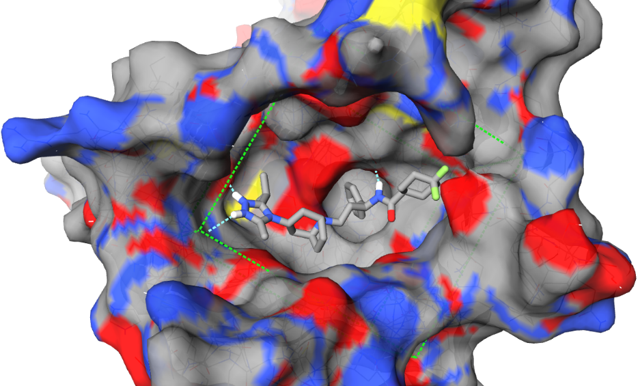
\includegraphics[width=0.48\linewidth]{../usrt/MRV0.png}
}
\subfloat[Orientational degree of freedom.]
{
  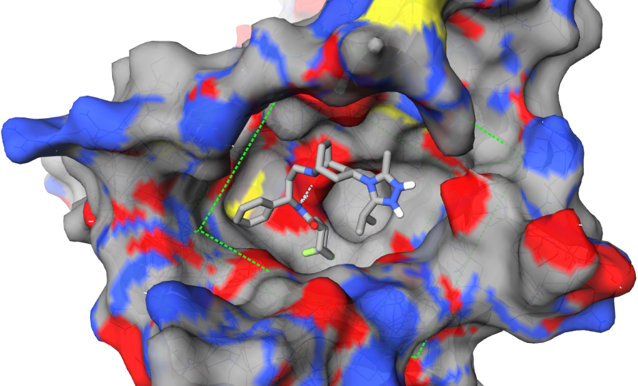
\includegraphics[width=0.48\linewidth]{../usrt/MRV1.png}
}
\caption{Two very different docked poses of the marketed HIV drug maraviroc in complex with the human CCR5 chemokine receptor (PDB: 4MBS). The protein is rendered in molecular surface representation. The ligand is rendered in stick representation. The binding cavity on the protein surface is depicted by a green cubic box. The putative intermolecular hydrogen bonds are shown as cyan dashed lines. The ligand poses were generated by idock \citep{1153} and the figure was rendered by iview \citep{1366}.}
\label{usr:MRV}
\end{figure}

\citep{1332} no shape method dominates when looking at each target individually, as each method is best in half of the targets. A wide range of factors collectively contribute to the large variability in performance observed across targets. First, errors in the generation of 3D conformers may impact differentially on the top ranked molecules depending on the query molecule and thus on the considered target.

Compared to other existing approaches \citep{1333,1334,1335,1337,1338,1331}, istar::USR has several distinctive features. First, it uses both USR and USRCAT. USR has an successful prospective application. USRCAT has an successful retrospective application. Second, it database has 23 million ZINC compounds. Third, it supports multiple queries in one job.

We choose USR \citep{1379} and USRCAT \citep{1331} because they have demonstrated pragmatic usefulness in prospective and retrospective virtual screening experiments, respectively.

\section{Methods}

\subsection{USR: ultrafast shape recognition}

The relative position of the atoms in the molecule is in turn completely determined by the set of all interatomic distances. This is a convenient representation, which directly eliminates any need for alignment or translation, as this set of distances is independent of molecular orientation or position.

the set of all interatomic distances contains more information that is needed to describe accurately the shape of the molecule. This is because the values of these distances are heavily constrained by the forces that hold the atoms together and thus using less information would still provide us with the discriminative power necessary to distinguish between molecules.

The goal is to find different compounds with a shape similar to that of the query, we will direct our attention to the four compounds with the highest score, instead of the four conformers with the highest score. The four conformers with the highest similarity score (top row) to the drug conformer APRD00001-1 from the DrugBank-3D database correspond to four conformations of the same compound, including the query. However, the reason why a database is populated with multiple conformers of each flexible compound is to reduce the possibility of missing compounds with similar shape to the query.

Four reference points, ctd: molecular centroid, cst: closest atom to ctd, fct: farthest atom to ctd, ftf: farthest atom to fct. Compute distances. Moments of these distances have semantics. For instance, the 1st, 2nd, 3rd moments of ctd capture the size, variance, skewness of the ligand, respectively. Applicable to different number of atoms. Dimension reduction: any ligand structure is mapped to a point in a 12 dimensional space. In combination with a suitable clustering algorithm, one could find clusters in a molecular database in order to select the most representative molecule of each cluster. The latter could be applied, for example, as a way to avoid repeating expensive biological tests on similar molecules.  This opens the door to the application of existing clustering algorithms to find groups of similar molecules as a way to analyse the molecular diversity of a database in terms of molecular shape. These roots are intended to provide all moments with linear space dimension, typically \AA, in order to avoid differences in high order moments overshadowing the contribution to the similarity score of low order moments.

\begin{equation}
m_1=\frac{1}{N}\sum_{l=1}^{N}d_i
\label{eqn:moment1}
\end{equation}

\begin{equation}
m_1=\frac{1}{N}\sum_{l=1}^{N}d_i
\label{eqn:moment2}
\end{equation}

\begin{equation}
m_1=\frac{1}{N}\sum_{l=1}^{N}d_i
\label{eqn:moment3}
\end{equation}

USRCAT computes the third moment in a different way. Our computation avoids overflow, and thus enables the distance distributions to contain only one sample. In this case the three moments will be all zeros.

Dissimilarity transformed into a normalized similarity score. (Eq \ref{eqn:usr}) Any inverse monotonic function can do.

\begin{equation}
S_{qi}=\frac{1}{1+\frac{1}{12}\sum_{l=1}^{12}|M_l^q-M_l^i|}
\label{eqn:usr}
\end{equation}

USR is highly extensible: changing reference points, as was done in \citep{1334,1335}, using higher orders of moments \citep{1333}.

\subsection{USRCAT: ultrafast shape recognition with CREDO atom types}

Atoms are partitions into subsets.
In the case of an empty subset, for examples if no hydrogen bond donors are found, then the corresponding elements in the moment vector will be set to zero.

\subsection{USR on istar}

Several levels of parallelism: multiple database ligands, multiple query ligands, multiple features.

Parallelized at the coarse grained level of a database of ligands to compare against.

AVX (Advanced Vector Extensions) instructions. Use PowerPoint to draw a diagram here to illustrate. unrolling, sub, abs, hadd.

All Clean Subset from ZINC (N=23,129,083)

Large 3D database, ZINC \citep{532,1178}, istar \citep{1362}, 23 million.
Like in istar::idock, we used the same database, for prospective screening.
Add figures here. The figures were rendered by iview \citep{1366}.
We will use RDKit to generate conformers \citep{1127} Freely Available Conformer Generation Methods: How Good Are They?

Time analysis: t = n(tq+ts)

\section{Conclusions}

USR has advantages in being independent of position and orientation.

Emphasize computational efficiency, 3 orders of magnitude faster than ESshape3D, and applicable to large-scale ligand database like istar \citep{1362}, which has collected 23 million ligands from ZINC \citep{532,1178}.

\section{Availability}

istar::USR is free and open source under Apache License 2.0. It is available at http://istar.cse.cuhk.edu.hk/usr.

\section{Future works}

USR is independent of position and orientation, but is dependent on torsions. Nevertheless, none of the above variants are independent of torsions. We present USRT, the first algorithm that is invariant of torsions. In the following sections, we describe USR and USRT, their effectiveness and efficiency.

We present the first algorithm that can distinguish ligands with different torsions. We call it USRT (Ultrafast Shape Recognition with Torsions). In USRT, the reference atom is chosen to be the atom connecting to the parent frame. It is BRANCH X Y, and is often the first of the current frame. For the ROOT frame, it is the first atom.

Figure \ref{usr:T27} shows two conformations with different torsions. This is a rotatable bond. This branch can rotate along the rotatable bond and flip to the right hand side. A torsion is the rotating angle, so it is in the range of -$\pi$ to $\pi$. 

\begin{figure}
\minipage{0.5\textwidth}
\centering
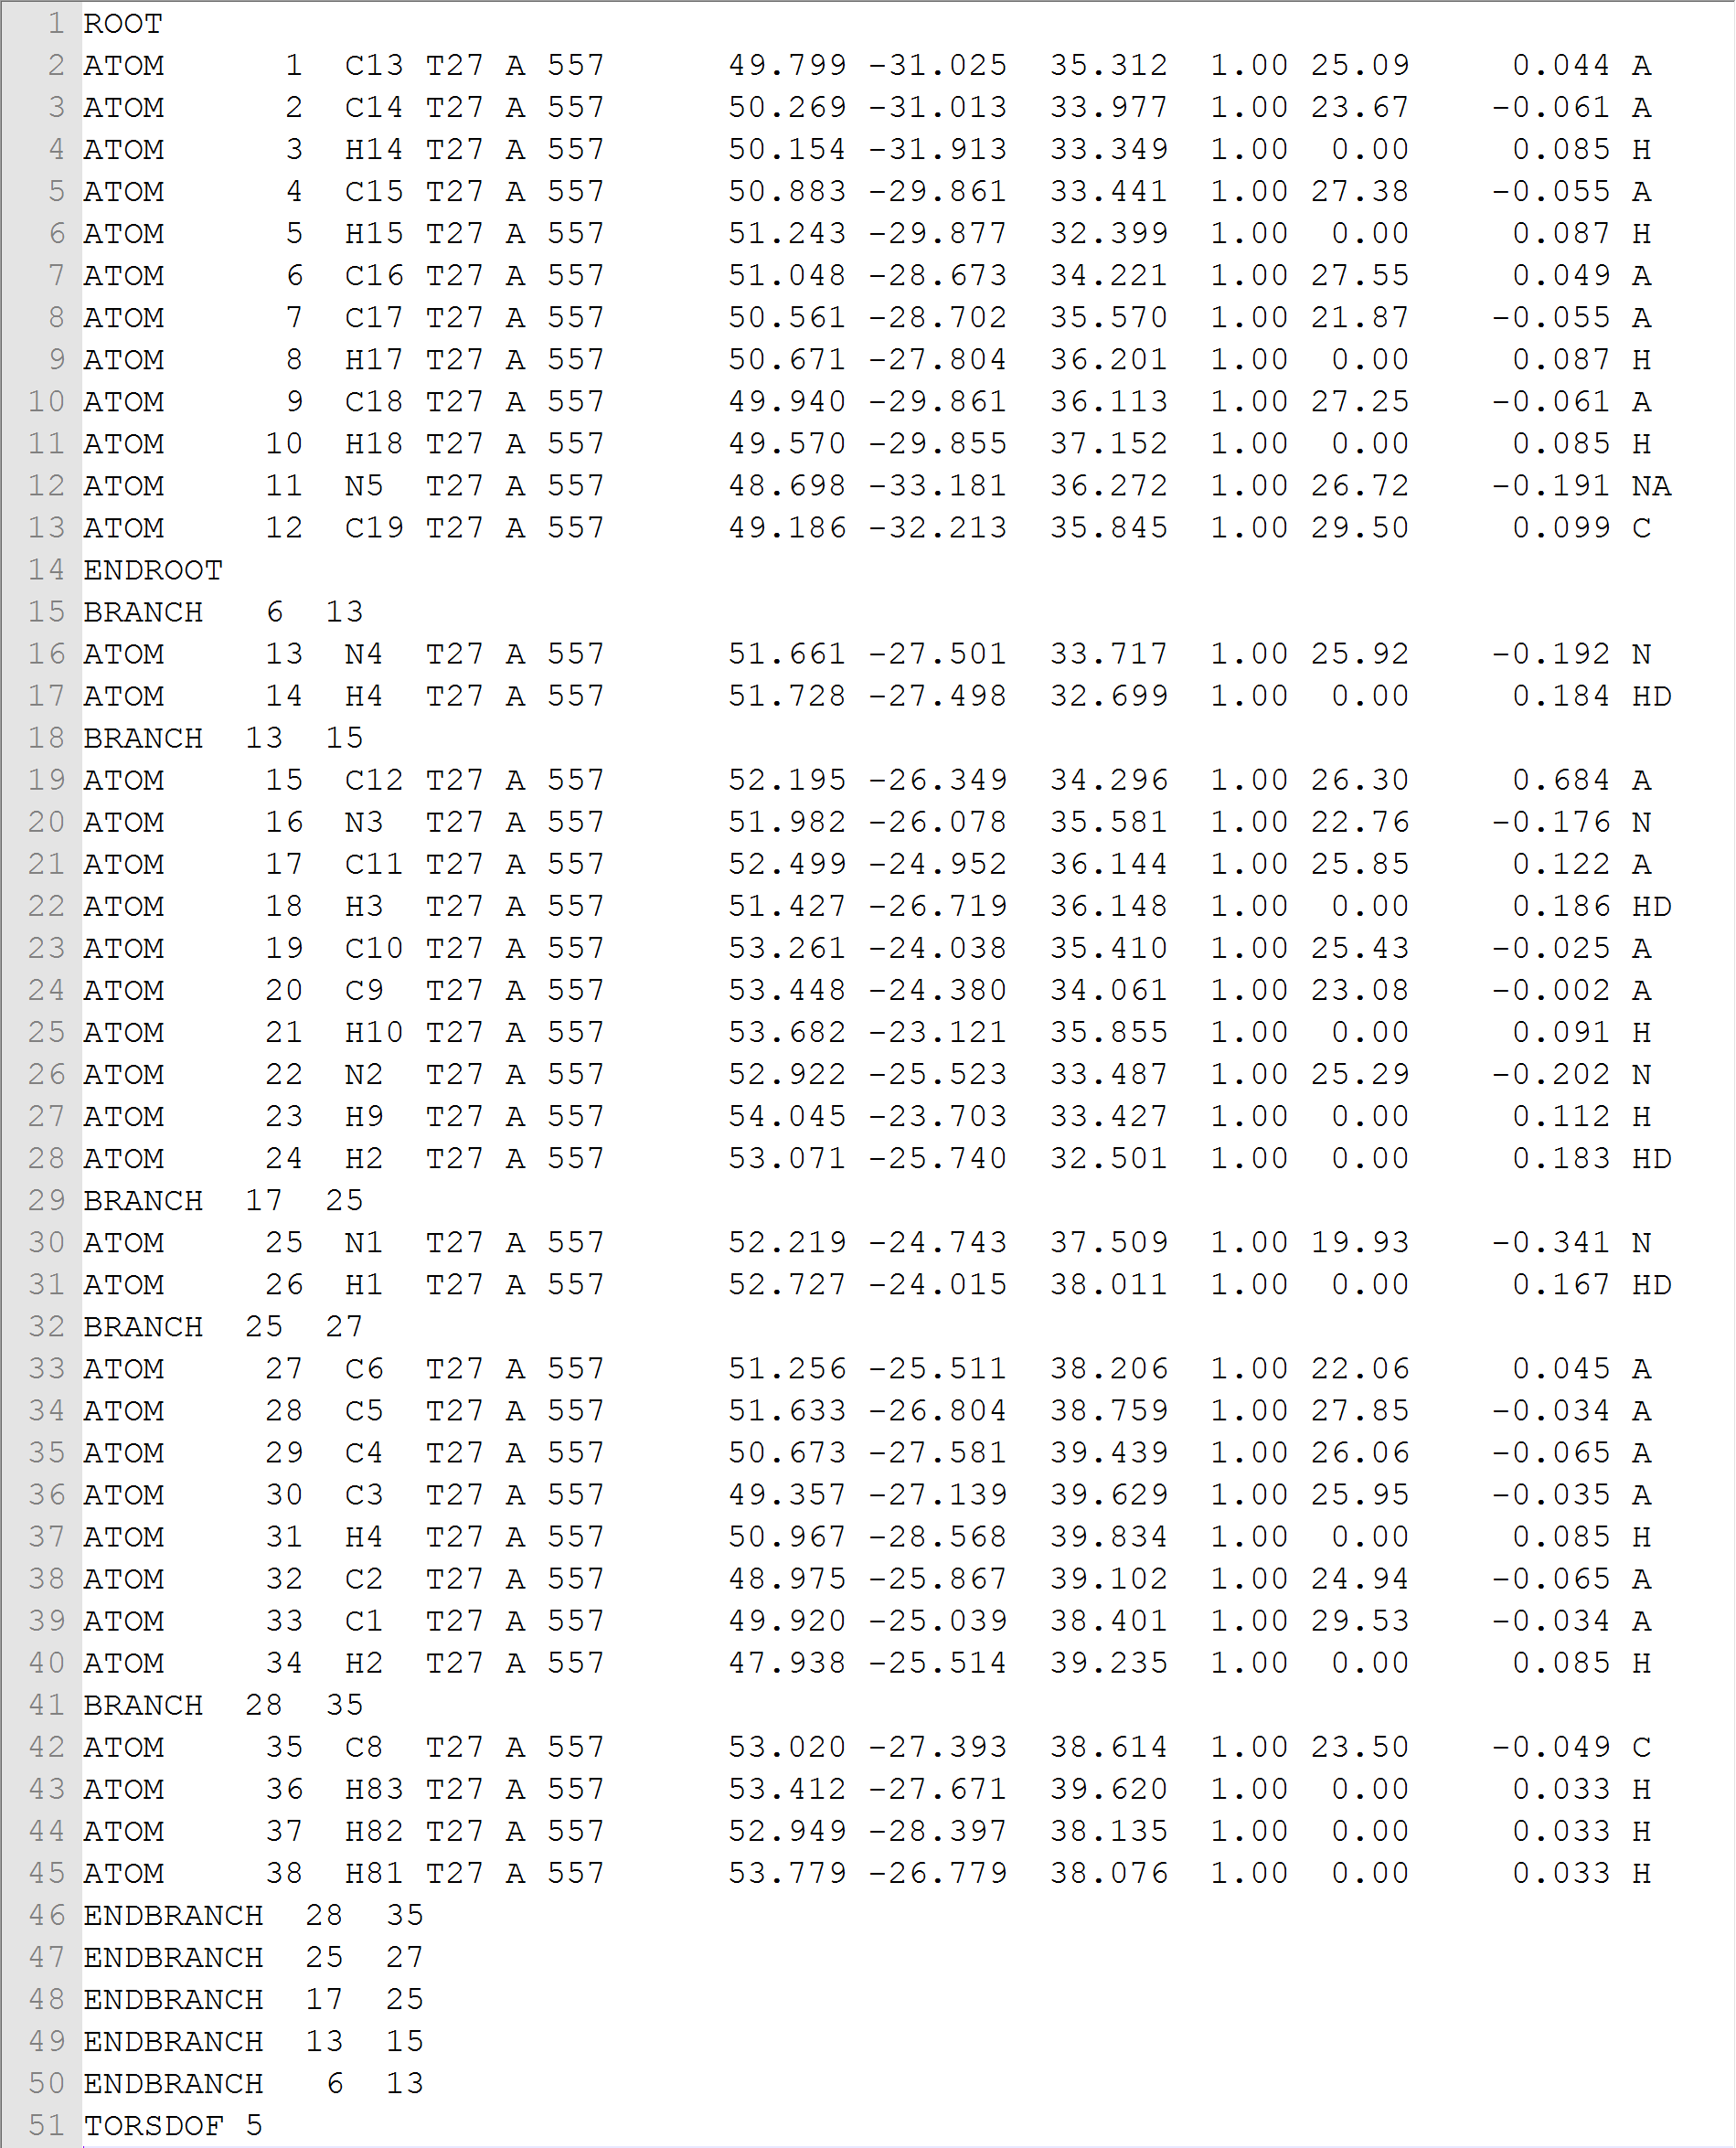
\includegraphics[width=1.36\textwidth,natwidth=1899,natheight=2350]{../usrt/T27CrystalPDBQT.png}
\endminipage
\minipage{0.5\textwidth}
\centering
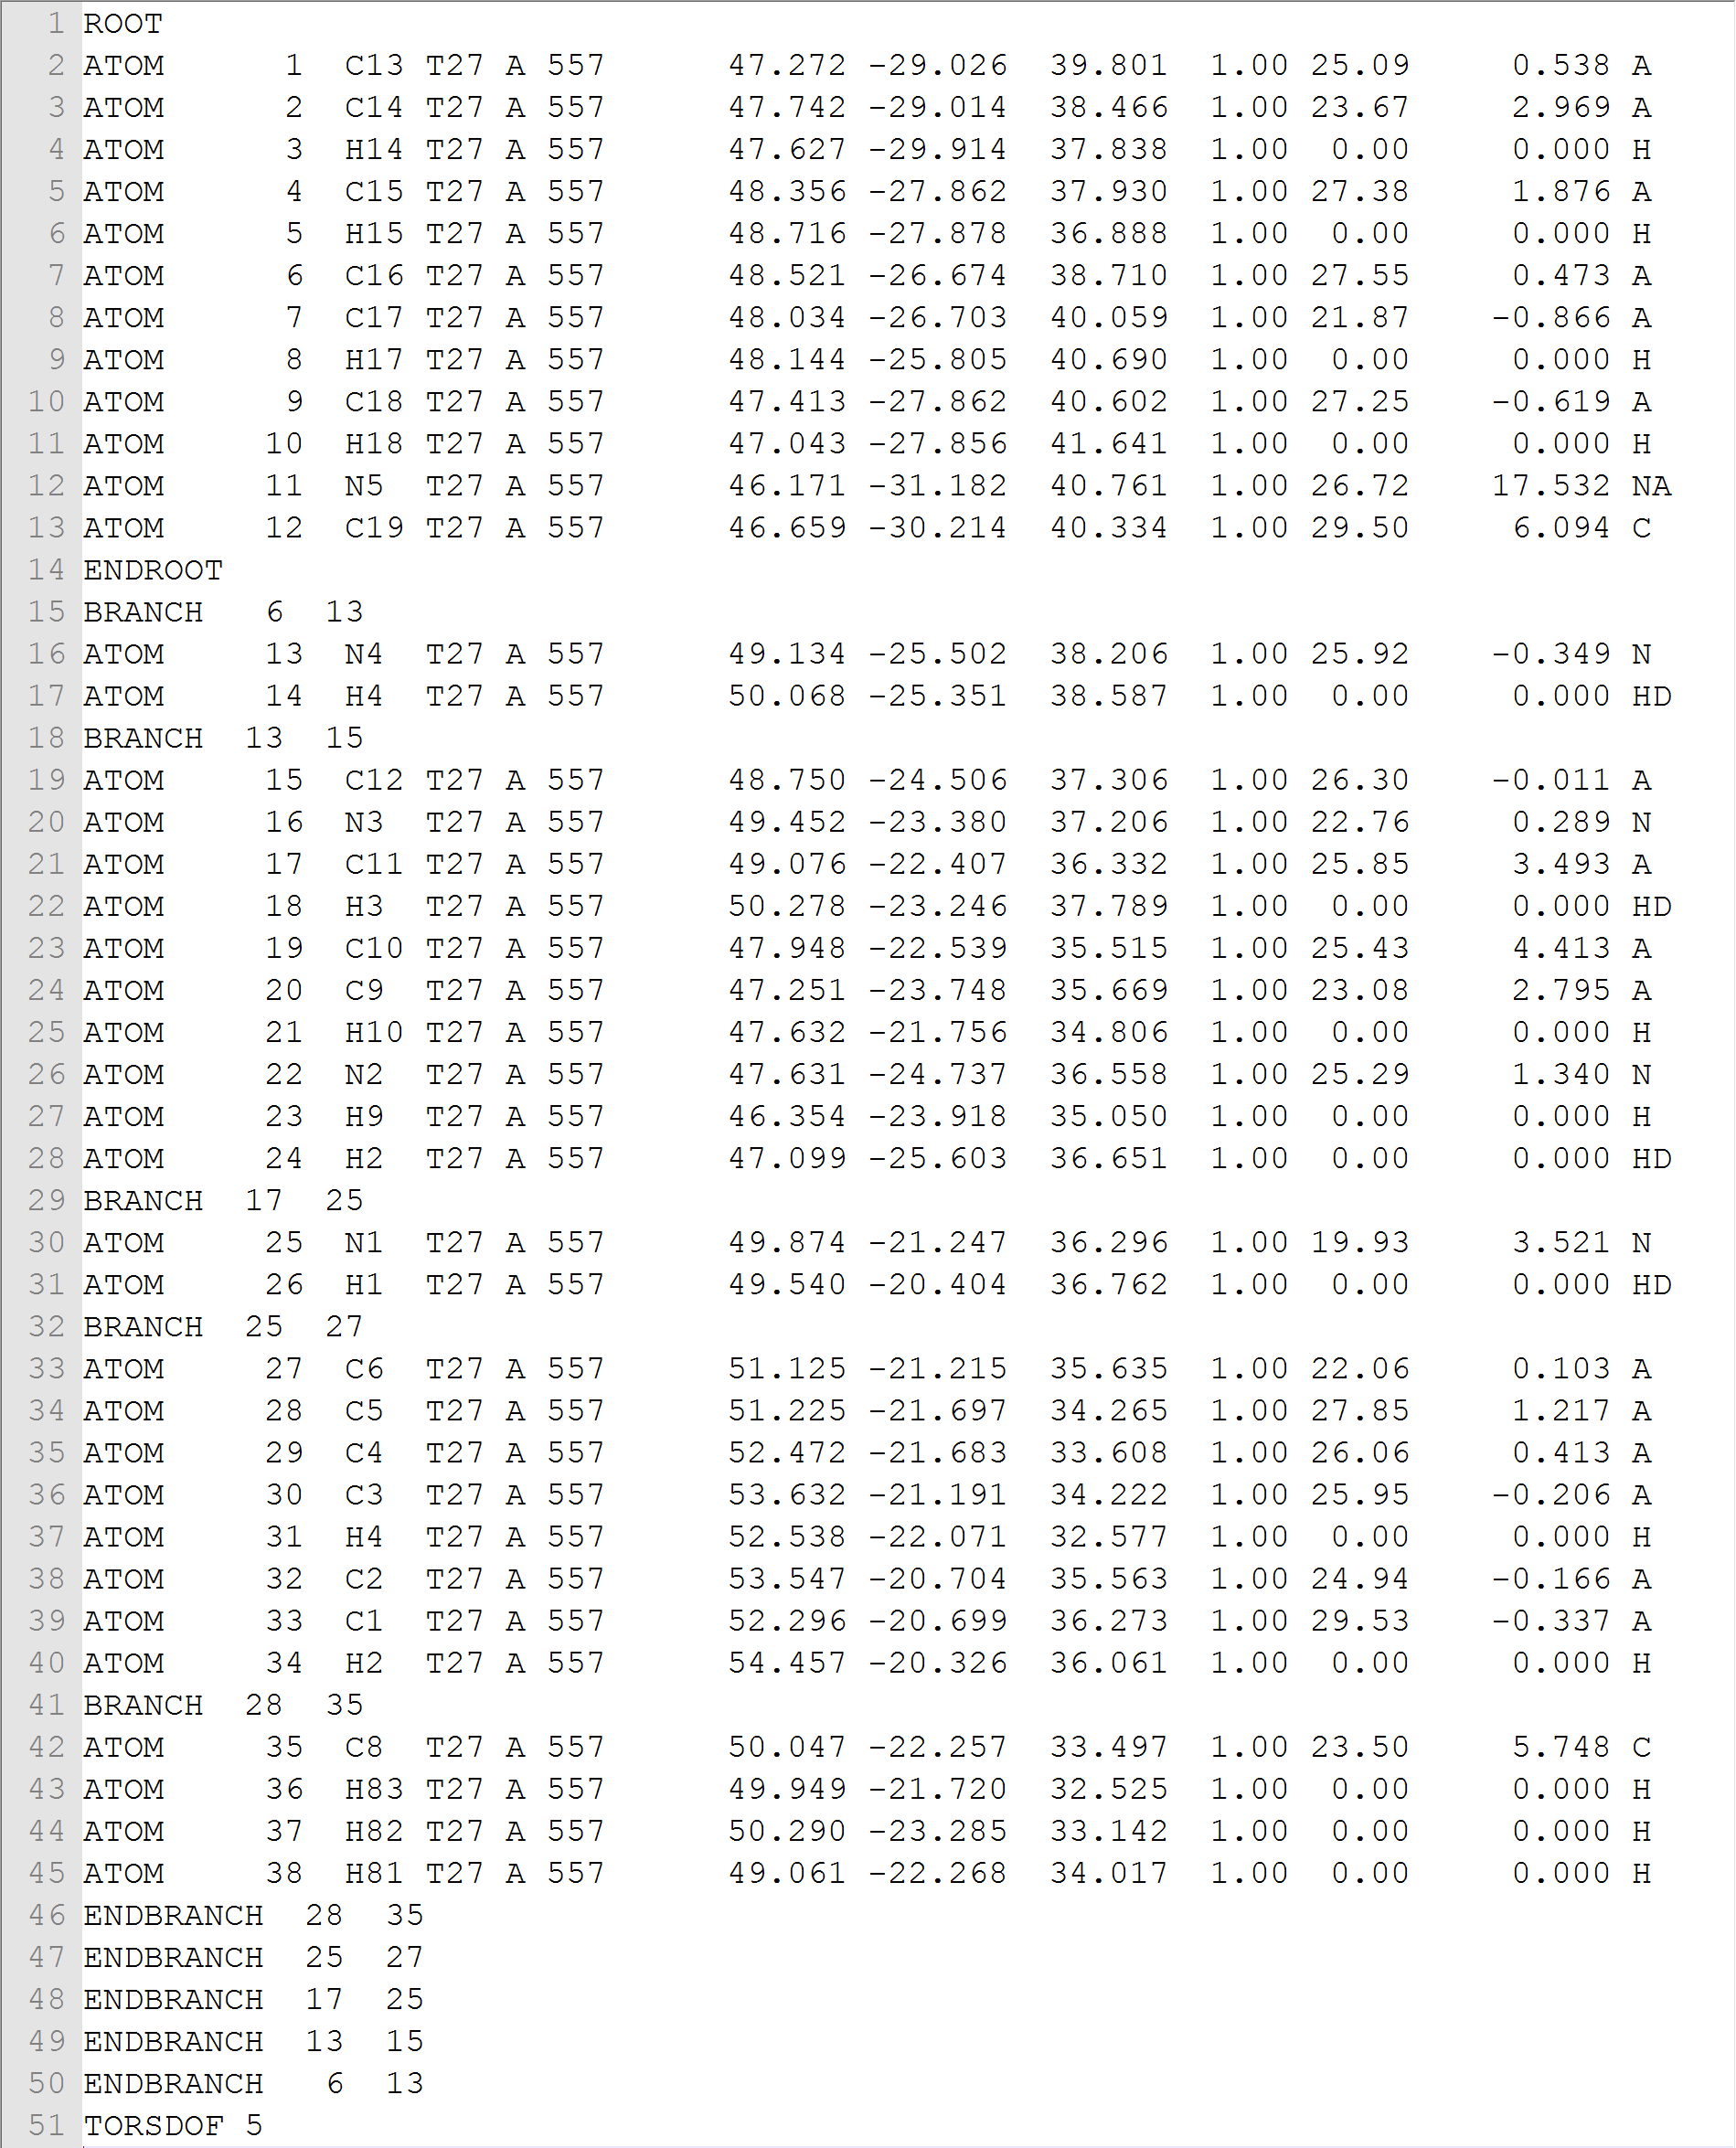
\includegraphics[width=1.36\textwidth,natwidth=1899,natheight=2350]{../usrt/T27DockedPDBQT.png}
\endminipage
\\
\minipage{0.5\textwidth}
\centering
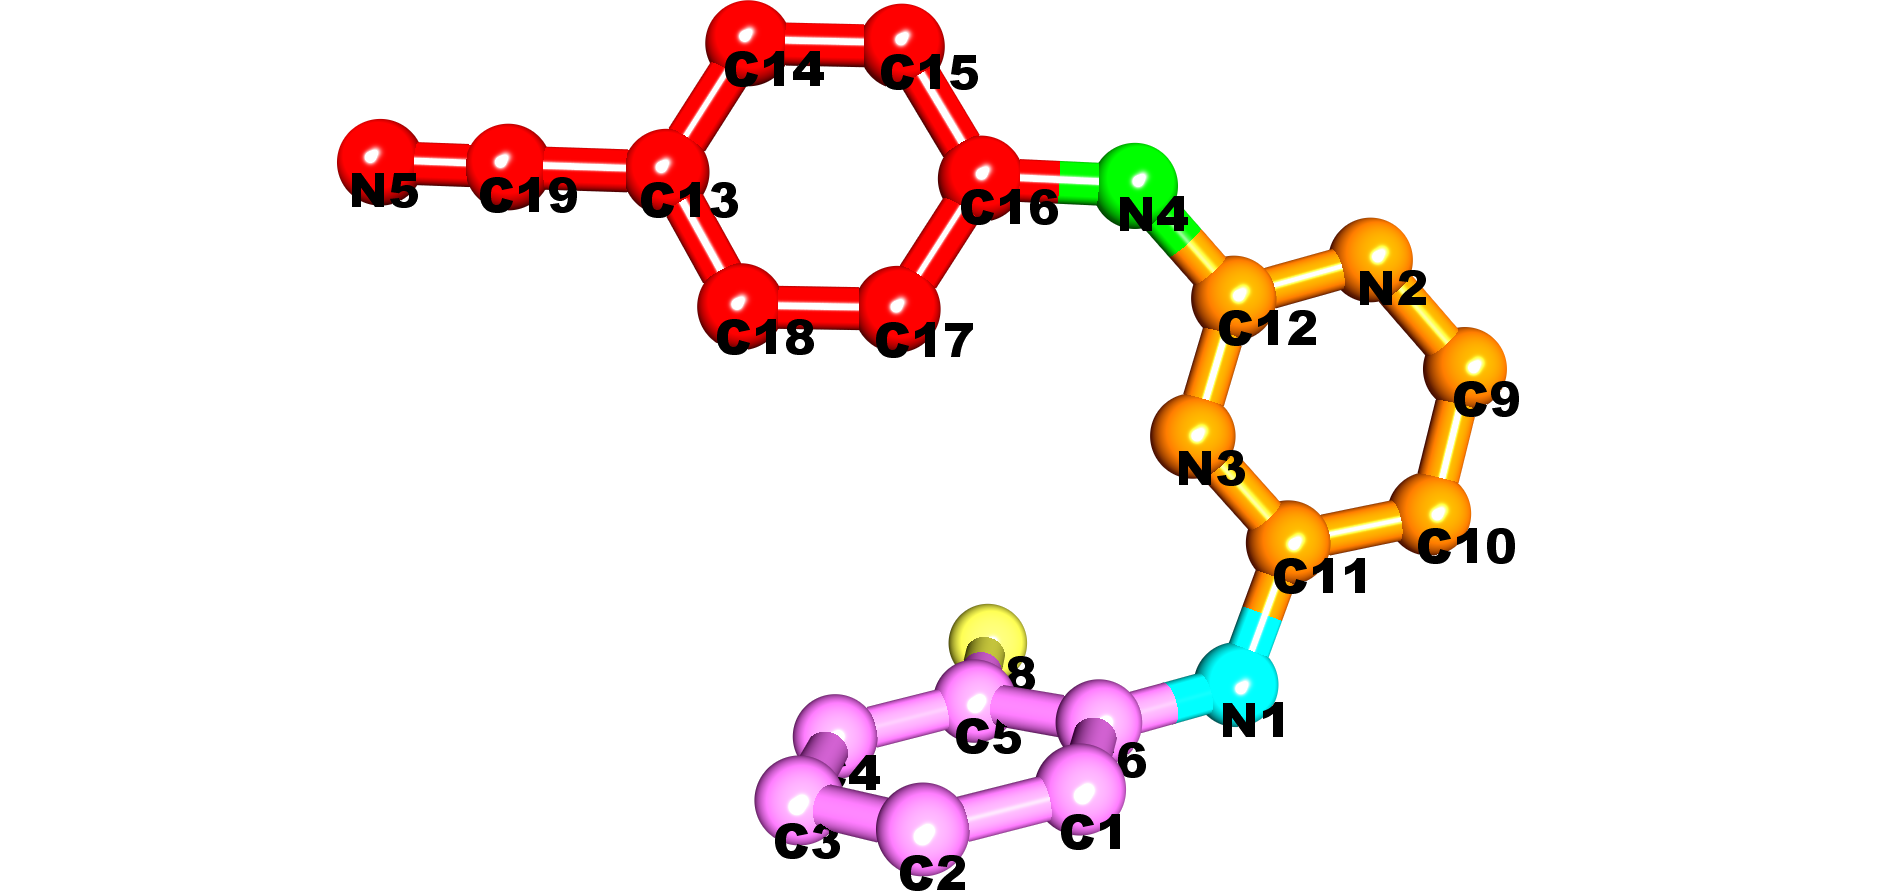
\includegraphics[width=1.36\textwidth,natwidth=1904,natheight=894]{../usrt/T27Crystal.png}
\endminipage
\minipage{0.5\textwidth}
\centering
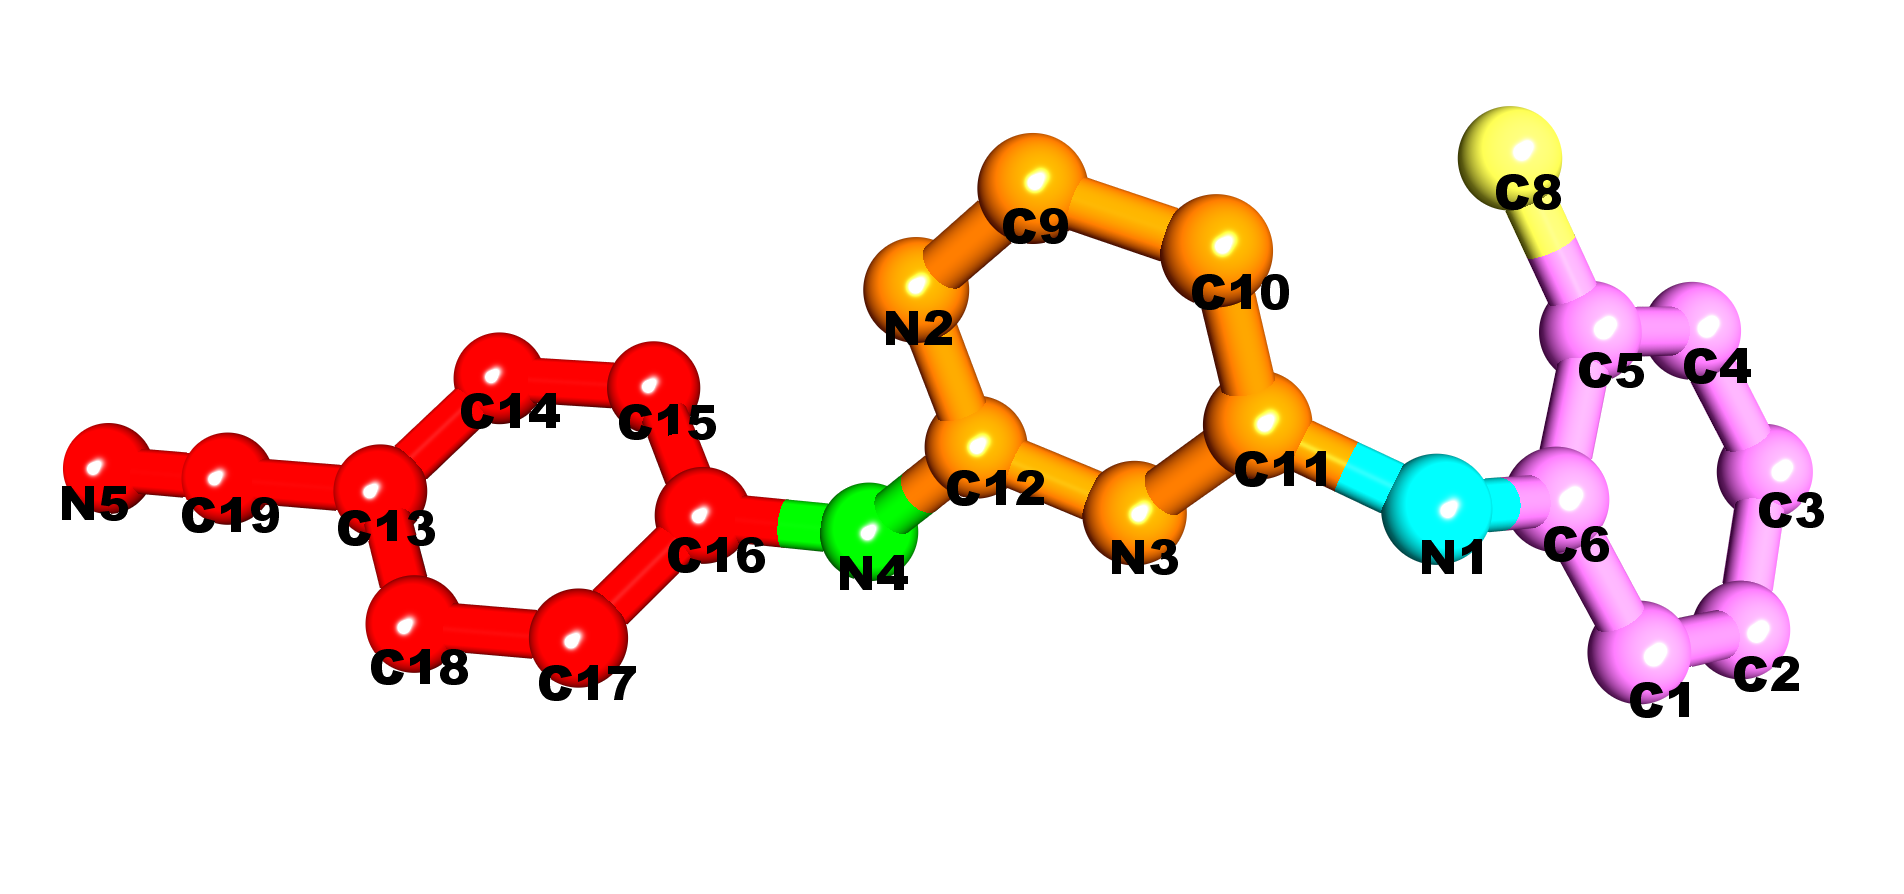
\includegraphics[width=1.36\textwidth,natwidth=1904,natheight=894]{../usrt/T27Docked.png}
\endminipage
\caption{Two very different poses of the same ligand, which has six frames and five rotatable bonds. Top row: the contents of the two poses in PDBQT format. Bottom row: the two poses in ball-and-stick representation. The atoms and bonds in the same frame are rendered in the same color.}
\label{usr:T27}
\end{figure*}

Once a reference atom is determined, the next is to compute inter-atom distances and their 1st, 2nd, 3rd moments. The output of USRT is a feature vector, which maps to a point in a high dimensional space. The length of the feature vector depends on the number of rotatable bonds. This format a natural clustering: the ligands having the same number of rotatable bonds are first categorized, and then all existing clustering algorithms can be utilized.

USRT inherits advantages from USR, like being ultrafast and extensible. It circumvents the need of aligning the molecules before testing for similarity. Compatible with USRCAT \citep{1331}, USR+MACCS \citep{1333} and possibly other USR variants \citep{1334}. can combine with other USR variants, e.g. USRCAT.

USRT is a general method that can be applied to various drug design applications, including de novo ligand deduplication and clustering. No conformers are required. the unbound bioactive conformation could be in principle significantly different from the corresponding bound conformation. No more considerations of using bound or unbound conformations.

Although very promising, major problems are: tree structure output, child frame matching, known ROOT frame, in-frame atom types, connector atom types. This raises the obvious question of how to compare molecules with different number of torsions, which are introduced by flexible ligand docking. Frames with less than 2 heavy atoms are ignored or assigned zero. Could be inactive frames like -CH3, -NH2 or -OH. Cannot compute 2nd and 3rd moments. Can incorporate connecting atoms of child branches. We will address the above limitations in future research using dynamic programming with frame insertion/deletion.

\chapterend
